\subsection{Plane Isometries}

This section studies groups through a geometric lens, specifically by looking at mappings of the Euclidean plane that preserve distance.


%%%%%%%%%%%%%%%%%%%%%%%%%%%%%%%%%%%%%%%%%%
%  Isometries and Their Group Structure  %
%%%%%%%%%%%%%%%%%%%%%%%%%%%%%%%%%%%%%%%%%%

\subsubsection{Isometries and Their Group Structure}

\Definition{Isometry}{
    An \textbf{isometry} of the Euclidean plane $\R^2$ is a permutation $\phi : \R^2 \to \R^2$ that preserves distance. That is, for any points $P, Q \in \R^2$, the distance between $P$ and $Q$ is equal to the distance between $\phi(P)$ and $\phi(Q)$.
}

\Theorem{}{
    The set of all isometries of $\R^2$ forms a subgroup of the group of all permutations of $\R^2$.
}

\Proof{
    The composition of two distance-preserving maps is distance-preserving. The identity map is an isometry. The inverse of an isometry is an isometry.
}

\Note{
    The group of isometries that carry a subset $S \subset \R^2$ onto itself is called the \textbf{symmetry group} of $S$. For a regular $n$-gon, this group is $D_n$.
}


%%%%%%%%%%%%%%%%%%%%%%%%%%%%%%%%%%%%%%%%
%  The Four Types of Plane Isometries  %
%%%%%%%%%%%%%%%%%%%%%%%%%%%%%%%%%%%%%%%%

\subsubsection{The Four Types of Plane Isometries}

It can be shown that every isometry of the plane is one of four types:
\begin{enumerate}
    \item \textbf{Translation $(\tau)$:} Slides every point by a fixed vector. \\
        Example: $\tau(x,y) = (x,y) + (2,-3) = (x+2,y-3)$
    \item \textbf{Rotation $(\rho)$:} Rotates the plane about a fixed point $P$. \\
        Example: $\rho(x,y) = (-y,x)$ is a rotation through $90^{\circ}$ counterclockwise about the origin.
    \item \textbf{Reflection $(\mu)$:} Reflects the plane across a fixed line $L$. \\
        Example: $\mu(x,y) = (x,-y)$ is a reflection across the $x$-axis.
    \item \textbf{Glide Reflection $(\gamma)$:} A reflection followed by a translation along the line of reflection. \\
        Example: $\gamma(x,y) = (x+1,-y)$ is a glide reflection across the $x$-axis followed by a translation of 1 unit to the right.
\end{enumerate}

\begin{figure}[htpb]
    \centering
    \begin{subfigure}{0.45\textwidth}
        \centering
        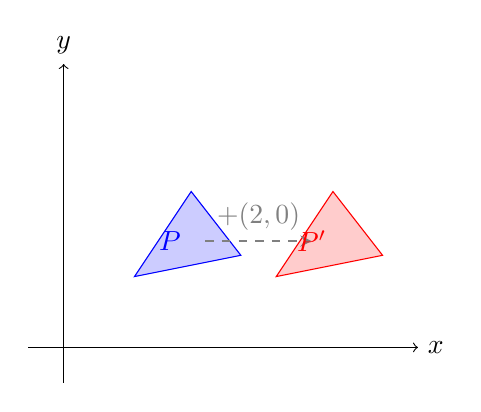
\begin{tikzpicture}[scale=0.9]
            \draw[->] (-0.5,0) -- (5,0) node[right] {$x$};
            \draw[->] (0,-0.5) -- (0,4) node[above] {$y$};
            \filldraw[blue, fill=blue!20] (1,1) -- (1.8,2.2) -- (2.5,1.3) -- cycle;
            \filldraw[red, fill=red!20] (3,1) -- (3.8,2.2) -- (4.5,1.3) -- cycle;
            \draw[->, gray, >=stealth, dashed, thick] (2,1.5) -- (3.5,1.5) node[midway, above] {$+(2,0)$};
            \node at (1.5,1.5) [blue] {$P$};
            \node at (3.5,1.5) [red] {$P'$};
        \end{tikzpicture}
        \caption{Translation: $\tau(x,y) = (x+2,y)$}
    \end{subfigure}
    \begin{subfigure}{0.45\textwidth}
        \centering
        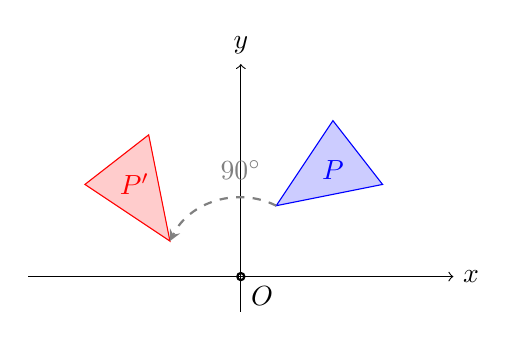
\begin{tikzpicture}[scale=0.9]
            \draw[->] (-3,0) -- (3,0) node[right] {$x$};
            \draw[->] (0,-0.5) -- (0,3) node[above] {$y$};
            \filldraw[blue, fill=blue!20] (0.5,1) -- (1.3,2.2) -- (2,1.3) -- cycle;
            \filldraw[red, fill=red!20] (-1,0.5) -- (-2.2,1.3) -- (-1.3,2) -- cycle;
            \draw[->, gray, >=stealth, dashed, thick] (0.5,1) arc (63.4:153.4:1.118);
            \draw[thick] (0,0) circle (0.05) node[below right] {$O$};
            \node at (1.3,1.5) [blue] {$P$};
            \node at (-1.5,1.3) [red] {$P'$};
            \node at (0, 1.5) [gray] {$90^{\circ}$};
        \end{tikzpicture}
        \caption{Rotation: $\rho(x,y)=(-y,x)$ about $O$}
    \end{subfigure}
    \begin{subfigure}{0.45\textwidth}
        \centering
        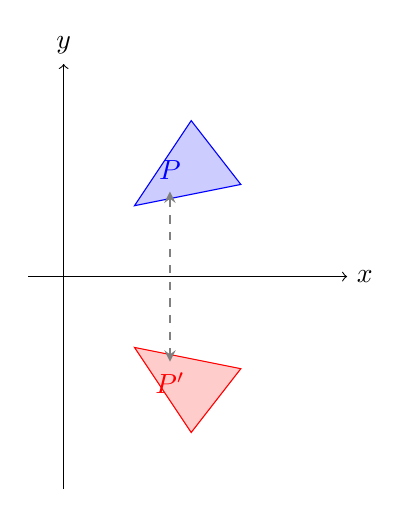
\begin{tikzpicture}[scale=0.9]
            \draw[->] (-0.5,0) -- (4,0) node[right] {$x$};
            \draw[->] (0,-3) -- (0,3) node[above] {$y$};
            \filldraw[blue, fill=blue!20] (1,1) -- (1.8,2.2) -- (2.5,1.3) -- cycle;
            \filldraw[red, fill=red!20] (1,-1) -- (1.8,-2.2) -- (2.5,-1.3) -- cycle;
            \node at (1.5,1.5) [blue] {$P$};
            \node at (1.5,-1.5) [red] {$P'$};
            \draw[<->, gray, >=stealth, dashed, thick] (1.5, 1.2) -- (1.5, -1.2);
        \end{tikzpicture}
        \caption{Reflection: $\mu(x,y)=(x,-y)$ across $x$-axis}
    \end{subfigure}
    \begin{subfigure}{0.45\textwidth}
        \centering
        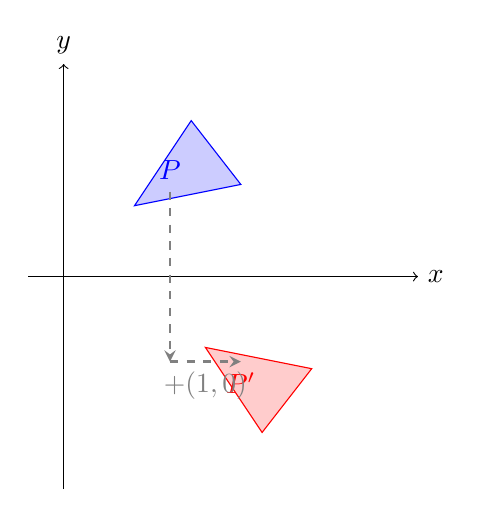
\begin{tikzpicture}[scale=0.9]
            \draw[->] (-0.5,0) -- (5,0) node[right] {$x$};
            \draw[->] (0,-3) -- (0,3) node[above] {$y$};
            \filldraw[blue, fill=blue!20] (1,1) -- (1.8,2.2) -- (2.5,1.3) -- cycle;
            \filldraw[red, fill=red!20] (2,-1) -- (2.8,-2.2) -- (3.5,-1.3) -- cycle;
            \node at (1.5,1.5) [blue] {$P$};
            \node at (2.5,-1.5) [red] {$P'$};
            \draw[->, gray, >=stealth, dashed, thick] (1.5, 1.2) -- (1.5, -1.2);
            \draw[->, gray, >=stealth, dashed, thick] (1.5, -1.2) -- (2.5, -1.2) node[midway, below] {$+(1,0)$};
        \end{tikzpicture}
        \caption{Glide reflection: $\gamma(x,y)=(x+1,-y)$}
    \end{subfigure}
    \caption{The four types of plane isometries}
    \label{fig:isometries}
\end{figure}

Isometries are classified as \textbf{orientation-preserving} (translations and rotations) or \textbf{orientation-reversing} (reflections and glide reflections). The orientation-preserving isometries form a subgroup of index 2 in any symmetry group that contains at least one orientation-reversing element.


%%%%%%%%%%%%%%%%%%%%%%%%%%%%
%  Finite Isometry Groups  %
%%%%%%%%%%%%%%%%%%%%%%%%%%%%

\subsubsection{Finite Isometry Groups}

The theorem below completely classifies the structures of finite subgroups of the full isometry group.

\Theorem{Leonardo's Theorem}{
    Every finite group $G$ of isometries of the plane is isomorphic to either:
    \begin{itemize}
        \item $\Z_n$, the cyclic group of order $n \ge 1$, consisting of rotations.
        \item $D_n$, the dihedral group of order $2n$ ($n \ge 1$), which includes the Klein 4-group when $n=2$.
    \end{itemize}
}

\Proof{
    We outline the proof by showing that there is a point in the plane fixed by every element of finite $G$. Let $G = \{\phi_1, \phi_2, \ldots, \phi_m\}$, and let $(x_i, y_i) = \phi_i(0,0)$ be the images of the origin under each isometry. Consider their \textbf{center of mass} $P = (\bar{x}, \bar{y})$: \[
        P = \left( \frac{x_1 + x_2 + \cdots + x_m}{m}, \frac{y_1 + y_2 + \cdots + y_m}{m} \right)
    \]
    The actions of isometries in $G$ merely permute the elements $\phi_i$ among themselves ($\phi_i \circ \phi_j = \phi_k$). Consequently, applying any $\phi \in G$ to the set of points $\{(x_i, y_i)\}$ simply permutes the points, leaving their center of mass $P$ unchanged. Therefore, $P$ is fixed by every isometry in $G$.
    
    The orientation-preserving isometries in $G$ must all be rotations about $P$ (or the identity). Since $G$ is finite, these rotations form a cyclic subgroup $\langle \rho \rangle \cong \Z_n$, where $\rho$ is the rotation through the smallest positive angle.
    
    If $G$ consists solely of orientation-preserving isometries, $G = \langle \rho \rangle \cong \Z_n$. If $G$ also contains an orientation-reversing isometry (a reflection across an axis passing through $P$), say $\mu$, then the elements of $G$ permute the vertices of a regular $n$-gon centered at $P$. Since the index of the rotation subgroup is 2, $G = \langle \rho \rangle \cup \mu \langle \rho \rangle$, which is isomorphic to the dihedral group $D_n$.
}


%%%%%%%%%%%%%%%%%%%%%%%%%%%%%%%%%%%%%%%%%%%%%%%%%%%%%
%  Infinite Isometry Groups: Friezes and Wallpaper  %
%%%%%%%%%%%%%%%%%%%%%%%%%%%%%%%%%%%%%%%%%%%%%%%%%%%%%

\subsubsection{Infinite Isometry Groups: Friezes and Wallpaper}

Beyond finite groups, we encounter groups of isometries describing patterns that repeat infinitely in one or two directions. These groups naturally arise in architecture, art, and crystallography.

\Definition{Discrete Frieze}{
    A \textbf{discrete frieze} consists of a pattern of finite width and height that is repeated endlessly in both directions along a baseline, forming an infinite strip (like a decorative border next to a ceiling).
}

All discrete frieze groups are infinite. Since the pattern repeats, there is always a minimal translation $\tau$ that slides the frieze to its next instance. This implies that every frieze group contains a subgroup generated by $\tau$, which is isomorphic to $\Z$.

\Example{Nonabelian Frieze Group $D_{\infty}$}{
    Consider an infinite sequence of integral signs spaced one unit apart: \[
        \dots \quad \int \quad \int \quad \int \quad \dots
    \]
    The symmetry group of this frieze is generated by a translation $\tau$ (one unit to the right) and a rotation $\rho$ of $180^{\circ}$ about the center of any integral sign. There are no reflections because of the asymmetry of the integral sign. Thus, the group is non-commutative, as $\tau\rho = \rho\tau^{-1}$. This resembles the rule in $D_n$, but $\tau$ has infinite order. We call this frieze group $D_{\infty}$.
}

\Example{Abelian Frieze Group $\Z \times \Z_2$}{
    Consider an infinite string of D's: \[
        \dots \text{ D D D D D } \dots
    \]
    Its group is generated by the translation $\tau$ and a horizontal reflection $\mu$ across a line cutting through the middle of the D's. Here, the generators commute: $\tau\mu = \mu\tau$. Hence, the group is abelian and isomorphic to $\Z \times \Z_2$.
}

\Note{
    In total, there are exactly \textbf{7 distinct types of discrete frieze groups}, classified by whether they admit horizontal reflections, vertical reflections, rotations, or non-trivial glide reflections.
}

If a pattern is repeated by translations along two non-parallel vector directions to fill the entire plane (like patterns on wallpaper or tiles on a floor), its symmetry group will contain a subgroup isomorphic to $\Z \times \Z$. 

\Note{
    It can be shown that there are exactly \textbf{17 different types of wallpaper groups} (or \textbf{plane crystallographic groups}) when classified according to the types of rotations, reflections, and glide reflections they admit.
}
